\section{Teori}
Jorda er omsluttet av et magnetfelt, som kan tilnærmes med en 
dipolorientert omtrent i flukt med rotasjonsaksen. Jordas magnetiske sørpol 
befinner seg i nærheten av jordas geografiske nordpol, og magnetisk nordpol 
befinner seg i nærheten av geografisk sørpol. Presiseringen "i nærheten av" 
er således viktig i forbindelse med dette prosjektet, ettersom dette gir 
opphav til fenomentet deklinasjon. Den magnetiske sørpolen befinner seg 
nemlig nord i Canada, og ikke ved nordpolen. Resultatet er at et magnetisk 
kompass vil orientere seg mot nord i Canada, og ikke mot geografisk nord, 
noe som kan forårsake problemer ved for eksempel navigasjon etter kompass. 
Denne misvisningen kalles deklinasjon og blir oppgitt som vinkelen mellom 
geografisk nord og retningen på magnetfeltet. På grunn av asymmetrien til 
de magnetiske polene i forhold til rotasjonsaksen, vil deklinasjonen 
variere og være avhengig av posisjonen på jorda.

Et annet fenomen er inklinasjon som sier noe om hvor mye magnetfeltet peker 
nedover. Ettersom magnetfeltlinjene ikke følger jordas overflate vil 
magnetfeltet peke i mer eller mindre grad nedover mot bakken. Inklinasjonen 
blir derfor oppgitt som den vertikale vinkelen mellom horisontalen og
magnetfeltet.

\subsection{Phyphox}
Phyphox er en app man kan laste ned på telefonen sin, som lar brukeren 
bruke telefonen sine sensorer til å foreta ulike målinger. Deriblant finnes 
det et magnetometer som lar en måle magnetfelt-styrken langs alle 
koordinataksene til telefonen, i tillegg til absolutt feltstyrke. Se 
\hyperlink{https://phyphox.org/sensors/}{https://phyphox.org/sensors/}
for mer informasjon om sensorer og koordinatsystemet til telefonen.

\subsection{Hvordan måle inklinasjonen}
For å måle inklinasjonen, trenger en kun å finne magnetfelt-styrken i horisontal-
planet og i vertikal retning. Da blir formelen for inklinasjonen slik:
\begin{equation}
    \gamma = \arctan \frac{-B_z}{B_H}
\end{equation}
Hvor $B_z$ er feltstyrken i z-retning, og $B_H$ er feltstyrken i horisontalplanet. 
Minustegnet foran $B_z$ kommer av at $B_z$ vil være en negativ størrelse, men vi 
ønsker en positiv vinkel for inklinasjonen. Når vi foretar målingene ved hjelp av 
phyphox får vi derimot ikke feltstyrken i planet eksplisitt, men i komponentform i 
x- og y-retning. Formelen vi kommer til å bruke blir dermed
\begin{equation}
    \gamma = \arctan{ \frac{-B_z}{\sqrt{B_x^2 + B_y^2}} }
\end{equation}
hvor $B_x$ og $B_y$ er henholdsvis magnetfeltstyrken i x- og y-retning.

\subsection{Hvordan måle deklinasjonen}
For å finne ut deklinasjonen kreves det at vi vet hvor både magnetisk sør og 
geografisk nord er, for så å kunne regne ut vinkelen mellom dem. For å oppnå dette, 
kan det benyttes et mellomsteg, et fast referansepunkt, som man relaterer både 
magnetfeltet og geografisk nord til. Hvis man så finner vinkelen mellom magnetfeltet 
og referansepunktet, og geografisk nord og referansepunktet, kan deklinasjonen 
regnes ut basert på dette. Gitt vinklene ovenfor blir deklinasjonen
\begin{equation}
    \alpha = \beta - \theta
\end{equation}
hvor $\beta$ er vinkelen mellom referansepunktet og magnetfeltet, og $\theta$ er 
vinkelen mellom referansepunktet og geografisk nord.

Vinkelen mellom referansepunktet og magnetfeltet kan bli funnet ved å sette opp 
telefonen sitt koordinatsystem slik at vinkelen mellom det og referansepunktet er 
kjent når en tar målingene. Gitt dette oppsettet blir vinkelen mellom magnetfeltet 
og koordinatsystemet
\begin{equation}
    \phi = \arctan \frac{B_y}{B_x}
\end{equation}
og dermed mellom referansepunktet og magnetfeltet
\begin{equation}
    \beta = \psi - \phi = \psi - \arctan \frac{B_y}{B_x}
\end{equation}
hvor $\phi$ er vinkelen mellom referansepunktet og koordinatsystemet.

\subsection{Posisjon Nidarosdomen, Tyholt}

\subsection{Geopy}

\begin{figure}
    \centering
    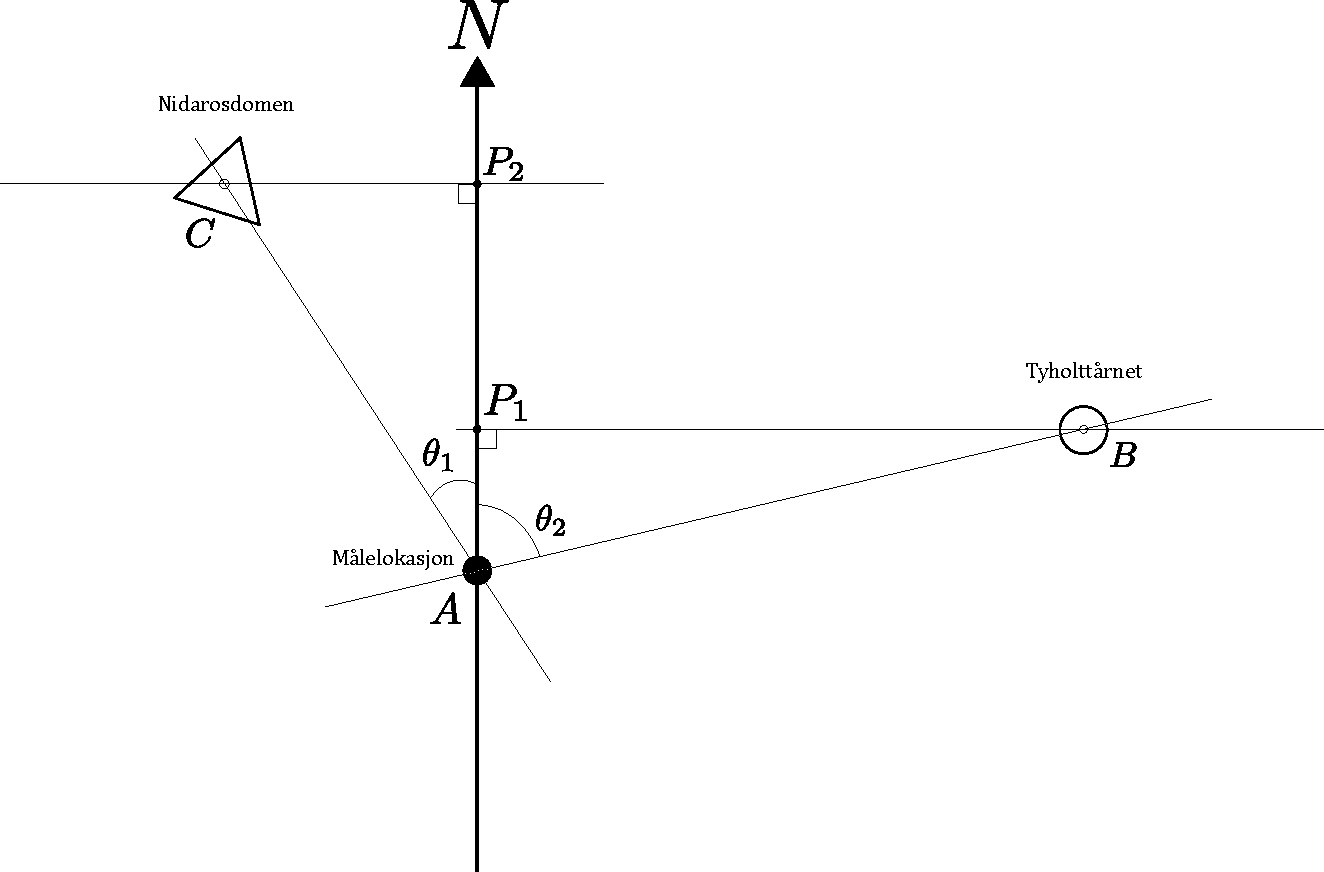
\includegraphics[width=\textwidth]{img/angle_north.pdf}
    \caption{Koordinatene til $B$ og $C$ blir estimert ved hjelp av Google Maps. 
    Koordinatene til målelokasjonen $A$ ble målt ved hjelp av Phyphox.
    $\theta_1$ og $\theta_2$ er vinklene hhv. vinkel mellom spiret på Nidarosdomen og nord, og mellom Tyholttårnet og nord. 
    Disse regnes ut ved å finne lengden til linjestykkene $\overline{AP_1}, \overline{BP_1}$ og $\overline{AP_2}, \overline{CP_2}$}.
    \label{fig:angle_north}
\end{figure}

For å finne vinkelen mellom referansepunktet og nord ser man på den rettvinklede trekanten med hjørner i målelokasjon, referansepunktet og et tredje punkt med samme lengdegrad som målelokasjonen og samme breddegrad som referansepunktet.
Tangens til $\theta$ er gitt ved $\overline{CP_2} / \overline{AP_2}$.
For å få riktig fortegn på vinkelen multipliseres det med $\text{sgn}(A_{\text{breddegrad}} - C_{\text{breddegrad}})$. Positiv vinkel blir da mot klokken sett ovenfra.
\par
For å regne ut avstandene ble python-biblioteket \textit{GeoPy} (\cite{geopy}) brukt. Funksjonen \kode{geopy.distance.distance} bruker en ellipsoidisk model av jordkloden (default: WGS-84) for å finne den korteste avstanden langs overflaten mellom to punkter (geodetisk kurve). 
 Denne funksjonen bruker \kode{Geodesic} fra biblioteket \kode{geographiclib} i bakgrunnen; en implementasjon av metoden gitt i Algorithms for geodesics (2013) \cite{Karney}. 



